\chapter{블랙홀, 화이트홀, 그리고 전역 인과도}

\lectureoverview{지평선은 국소적으로는 평범하지만 전역적으로는 결정적이다. 지평선 근처의 슈바르츠실트 계량에서 출발해 유클리드 시가 비유를 이용해 바깥쪽으로 살펴본 다음, 앨리스와 밥이 실제로 무엇을 볼 수 있는지 묻는다. 특이점과 시간 반전된 화이트홀 영역은 이 국소적 그림을 영원한 슈바르츠실트 시공간으로 확장한다. 펜로즈 압축을 적용하면 인과 구조가 유한한 영역에 들어와 읽기 쉬워진다. 마지막으로 영원한 해에서 붕괴로 형성된 블랙홀로 논의를 옮긴다. 이때 뉴턴의 껍질 정리와 버코프 정리가 이어 붙일 부분들을 제공한다.}

\section{지평선에서 무한대까지}

충분히 큰 슈바르츠실트 블랙홀의 지평선 근처에서는 작은 실험실 영역의 곡률이 약하므로, 반지름과 시간으로 이루어진 기하학은 거의 평탄하다. 편리한 반지름 변수는 슈바르츠실트 좌표 \(r\)가 아니라, 시간 일정한 공간 절편을 따라 지평선에서 바깥쪽으로 잰 고유거리 \(\rho\)이다:
\begin{equation}
\rho=0 \quad\Longleftrightarrow\quad r=2GM .
\label{eq:l04-rho-horizon}
\end{equation}
편리한 시간 좌표는 무차원량
\begin{equation}
\omega=\frac{t}{4GM},
\label{eq:l04-omega}
\end{equation}
이다. 여기서 \(c=1\)이다. 따라서 \(\omega\)는 슈바르츠실트 시간을 슈바르츠실트 반지름의 2배를 단위로 나타낸 것이다.

부호 규약을 대부분 양수로 두면 지평선 근처의 반지름-시간 계량은
\begin{equation}
ds^2\approx-\rho^2d\omega^2+d\rho^2.
\label{eq:l04-rindler}
\end{equation}
이다. 현재 논의는 시간과 반지름 거리에만 관련되므로 각방향의 2차원 구면은 생략했다.

\begin{figure}[htbp]
\centering
\includegraphics[width=0.72\textwidth]{lecture_04_figure_02.png}
\caption{지평선 근처의 계량과 재척도화한 슈바르츠실트 시간.}
\lectureframe{00:05:46.800}
\end{figure}

식~\eqref{eq:l04-rindler}은 민코프스키 시공간과 극좌표계의 유클리드 평면 사이의 관계와 같다. 다음과 같이 두면
\begin{equation}
T=\rho\sinh\omega,
\qquad
X=\rho\cosh\omega,
\end{equation}
다음 식을 얻는다.
\begin{equation}
-dT^2+dX^2=-\rho^2d\omega^2+d\rho^2.
\end{equation}
\(\rho\)가 일정한 선은 쌍곡선 \(X^2-T^2=\rho^2\)이고, \(\omega\)는 먼 과거에서 먼 미래까지 이어진다. 두 영선 \(X=\pm T\)는 축약한 도표에서 쌍극점에서 만난다. 4차원에서 이 점은 2차원 구면을 나타내며, 미래와 과거의 두 영시트는 분기 킬링 지평선을 이룬다.\editorialnote{반지름 도표에서는 교차점만을 분기 지평선이라고 부르는 것이 유용한 약칭이다. 더 정확히 말하면 두 지평선 가지는 분기 2차원 구면에서 교차한다.}

\subsection{먼 영역}

슈바르츠실트 계량의 반지름-시간 부분은
\begin{equation}
ds^2
=-\left(1-\frac{2GM}{r}\right)dt^2
+\frac{dr^2}{1-\frac{2GM}{r}}.
\label{eq:l04-schwarzschild}
\end{equation}
이다. 블랙홀에서 멀리 떨어진 곳, 즉 \(r\gg2GM\)에서는 계량이 다음에 가까워진다.
\begin{equation}
ds^2\approx-dt^2+dr^2.
\end{equation}
이 영역에서는 \(r\)와 \(\rho\)가 본질적이지 않은 덧셈 보정만큼만 다르므로, \(dt=4GM\,d\omega\)를 사용하면
\begin{equation}
ds^2\approx-(4GM)^2d\omega^2+d\rho^2.
\label{eq:l04-far}
\end{equation}
반지름 계수는 두 극한에서 모두 단순하다. 달라지는 것은 시간 계수다.
\begin{equation}
ds^2\approx
\begin{cases}
-\rho^2d\omega^2+d\rho^2, & \rho\ll GM,\\[3pt]
-(4GM)^2d\omega^2+d\rho^2, & \rho\gg GM.
\end{cases}
\label{eq:l04-two-limits}
\end{equation}
정지 궤적을 따라서는 \(d\rho=0\)이다. 지평선 가까이에서는
\begin{equation}
d\tau=\rho\,d\omega,
\end{equation}
인 반면, 멀리서는 \(d\tau\approx4GM\,d\omega=dt\)이다. 외부 시간 좌표가 같은 만큼 변해도 지평선에 가까운 곳에 둔 시계에서는 점점 더 짧은 고유시간이 흐른다.

\subsection{시가}

시공간은 머릿속에 그리기 어려우므로, 시간꼴 방향을 보통의 각방향으로 바꿔 보자. 다음과 같이 쓴다.
\begin{equation}
\begin{aligned}
d\ell^2&=F(\rho)^2d\theta^2+d\rho^2,\\
F(\rho)&\sim
\begin{cases}
\rho, & \rho\to0,\\
4GM, & \rho\to\infty.
\end{cases}
\end{aligned}
\label{eq:l04-cigar}
\end{equation}
\(\rho=0\) 근처에서는 극좌표로 나타낸 평면이다. 멀리서는 원둘레가 더 이상 반지름에 따라 커지지 않는다.
\begin{equation}
C_\infty=\int_0^{2\pi}4GM\,d\theta=8\pi GM.
\label{eq:l04-cigar-circumference}
\end{equation}
따라서 이 곡면은 한쪽 끝에서 둥글게 닫히고, 다른 쪽에서는 원통에 가까워진다. 시가처럼 보인다.

\begin{figure}[htbp]
\centering
\includegraphics[width=0.74\textwidth]{lecture_04_figure_03.png}
\caption{유클리드 기하의 비유: 극좌표의 끝점과 점근 원통을 잇는 곡면. 원통의 원둘레는 \(8\pi GM\)이다.}
\lectureframe{00:14:05.000}
\end{figure}

질량이 클수록 점근 영역의 둘레가 크고 끝점 근처의 굴곡은 완만하다. 작은 블랙홀은 굴곡이 심한 시가에 해당하고, 큰 블랙홀은 폭이 넓고 곡률이 약한 끝점을 갖는다. 이는 식~\eqref{eq:l04-two-limits}에서 보간되는 양을 나타낸 그림이지, 로런츠 블랙홀 자체를 매장한 그림은 아니다.\editorialnote{정확한 기하학적 대상은 슈바르츠실트 시간을 허수 시간으로 해석 연장해 얻는다. 그러면 끝점에서의 매끄러움이 유클리드 시간의 주기를 \(8\pi GM\)로 정하는데, 이는 뒤에 호킹 온도를 결정하는 것과 같은 척도다. 여기서는 시각적 비유로만 사용한다.}

\section{인과적으로 보는 지평선}

블랙홀 바깥 \(\rho>0\)에서 정지 관측자는 \(\rho\)가 일정한 쌍곡선을 따른다. 멀리서는 중력에 저항하는 데 필요한 가속도가 크지 않지만, 지평선 가까이에서는 필요한 고유가속도가 무한히 커진다. 세계선이 미래 영경계를 지나면, 그 세계선에서 나온 미래지향 인과 신호는 어느 것도 외부에 도달할 수 없다.

\begin{classroomqa}
\audiencequestion{이 도표에서 광선은 직선인가요?\lecturetimestamp{00:20:21}}
\lecturerresponse{다른 규약을 명시하지 않는 한, 반지름 방향 광선은 \(45^\circ\)로 그린다. 안쪽으로 향하는 광선은 지평선을 통과하지만, 이미 내부에 있는 바깥쪽 방향 광선은 외부로 되돌아갈 수 없다.}
\end{classroomqa}

\begin{classroomqa}
\audiencequestion{안쪽으로 들어가는 광선은 지평선에 계속 머무르나요?\lecturetimestamp{00:21:12}}
\lecturerresponse{아니다. 안쪽을 향하는 광선은 미래 지평선을 통과해 블랙홀 내부로 계속 나아간다. 영 경계에 머무르는 것은 지평선 생성선 자체뿐이다.}
\end{classroomqa}

\subsection{밥은 앨리스를 어떻게 볼까}

밥은 일정한 반지름에서 블랙홀 바깥에 머물고, 앨리스는 안쪽으로 떨어진다고 하자. 밥은 앨리스에게서 바깥쪽으로 오는 빛을 받아야만 그녀를 볼 수 있다. 앨리스가 자신의 시계에 따라 주기적으로 손을 흔든다고 하자. 그녀가 낙하하는 동안 나중에 방출한 신호일수록 밥에게 도달하는 데 슈바르츠실트 시간이 점점 더 오래 걸리고, 밥은 단위 시간당 더 적은 수의 파동을 받는다. 지평선을 지난 뒤 방출된 신호는 밥에게 돌아올 수 없다.

린들러 좌표를 이용하면 이 극한 거동을 드러낼 수 있다. 바깥쪽 영좌표를 다음과 같이 정의한다.
\begin{equation}
U=T-X=-\rho e^{-\omega}.
\end{equation}
미래 지평선에 다가간다는 것은 \(U\to0^{-}\)을 뜻하며, 외부의 \(\rho\)가 고정되어 있으려면 \(\omega\to+\infty\)이어야 한다. 따라서 앨리스가 유한한 시간에 지평선을 통과하는 사건은 외부 시간으로 무한대에 밀려난다. 연이어 도착하는 파동 마루 사이의 간격은 지수적으로 늘어나므로 주파수는 지수적으로 적색편이된다.\editorialnote{이 영좌표 계산은 강의에서 정성적으로 설명한 적색편이 현상을 수학적으로 나타낸다. 여기서는 국소 린들러 근사만 사용한다.}

처음에 밥은 가시광선을 받다가 적외선, 그리고 파장이 엄청나게 긴 전파를 받는다. 앨리스가 지평선 위에 영원히 보이는 사진처럼 남는다고 말하는 것은 적절하지 않다. 그녀는 점점 희미해지고 붉게 보이다가 결국 감지할 수 없게 된다.

\begin{classroomqa}
\audiencequestion{밥은 앨리스가 지평선 바깥의 한 정확한 위치에 멈춰 있는 모습을 보나요?\lecturetimestamp{00:26:31}}
\lecturerresponse{고전적인 외부 좌표로 기술하면, 점점 더 늦은 시각에 관측되는 영상은 지평선에 점점 더 가까운 사건에서 온다. 극한에서 영상은 그곳에 멈춰 있는 것처럼 보이지만, 복사는 적색편이되어 사실상 사라진다. 이 설명에는 아직 블랙홀의 양자물리가 포함되지 않는다.}
\end{classroomqa}

\begin{classroomqa}
\audiencequestion{앨리스가 희미해지는 동안, 몸이 압축되어 보이기도 하나요?\lecturetimestamp{00:28:34}}
\lecturerresponse{그렇다. 외부에서 기술할 때 상대운동으로 인해 길이 방향 로런츠 수축이 생긴다. 여기서 관측상 중요한 효과는 여전히 적색편이다. 앨리스의 내부 진동은 더 느려 보이고, 수신되는 파장은 길어진다.}
\end{classroomqa}

\subsection{앨리스는 밥을 어떻게 볼까}

앨리스의 고유시간은 지평선에서 규칙적으로 흐른다. 밥이 보내는 신호는 앨리스와 같은 인과 방향을 따라오므로, 앨리스는 지평선을 통과한 뒤에도 안쪽으로 오는 신호를 계속 받는다. 내부로 들어간 앨리스는 외부로 답신을 보낼 수 없다. 지평선은 한쪽 방향으로만 통과할 수 있는 경계이지, 양쪽에서 대칭적으로 마주치는 벽이 아니다.

\begin{classroomqa}
\audiencequestion{앨리스는 낙하하며 밥의 빛이 청색편이된 것을 보나요?\lecturetimestamp{00:30:29}}
\lecturerresponse{여기서 사용한 그림에서는 앨리스에게서 멀어지는 밥이 보이고, 밥의 신호는 적색 쪽으로 이동한다. 앨리스가 지평선을 통과할 때 특이한 일은 일어나지 않는다. 정확한 주파수 변화는 두 세계선과 밥이 신호를 방출하는 시점 모두에 달려 있다. 따라서 불변적으로 말할 수 있는 것은 규칙적인 지평선에서 앨리스가 측정하는 주파수가 유한하다는 점이다.}
\end{classroomqa}

\begin{classroomqa}
\audiencequestion{같은 인과적 제한이 중력자에도 적용되나요?\lecturetimestamp{00:31:15}}
\lecturerresponse{실제 중력 복사에도 광자와 똑같이 적용된다. 미래 지평선 뒤에서 방출된 복사 교란은 밥에게 도달할 수 없다.}
\end{classroomqa}

\begin{classroomqa}
\audiencequestion{앨리스가 블랙홀로 떨어지면 그녀의 에너지가 블랙홀의 질량과 반지름을 늘리나요?\lecturetimestamp{00:31:43}}
\lecturerresponse{그렇다. 앨리스의 에너지가 블랙홀에 포함되면 그 질량이 커지고 슈바르츠실트 반지름 \(R_s=2GM\)도 함께 커진다. 블랙홀의 동역학적 형성을 다루면 이 진술을 기하학적으로 설명할 수 있다.}
\end{classroomqa}

\subsection{외부에도 중력이 있는 이유}

블랙홀은 어둡지만 중력이 없는 것은 아니다. 정적인 중력장은 내부에서 끊임없이 빠져나오는 온셸 중력자의 흐름이 아니다. 이미 형성되어 있는 외부 기하학이다. 원천이 변하면 그에 따른 장의 변화는 인과적으로 전파되므로, 멀리 있는 관측자는 빛 신호가 도달할 수 있는 시점보다 먼저 그 변화를 감지할 수 없다.

\begin{classroomqa}
\audiencequestion{중력자가 빠져나올 수 없다면 블랙홀은 어떻게 중력을 작용시키나요?\lecturetimestamp{00:32:04}}
\lecturerresponse{정적 장은 이미 외부에 존재한다. 이를 가상 중력자를 이용해 느슨하게 설명할 수는 있지만, 가상 중력자는 내부에서 새로운 메시지를 전달하는 검출 가능한 입자가 아니다. 빛의 속도로 제한되는 것은 중력 복사를 비롯해 장에서 일어나는 변화다.}
\end{classroomqa}

\begin{classroomqa}
\audiencequestion{가상 중력자가 빛보다 빠를 수 있다는 말은 장의 변화가 빛의 속도로 전파된다는 진술과 어떻게 양립하나요?\lecturetimestamp{00:34:02}}
\lecturerresponse{가상 양자는 섭동 계산에서 쓰이는 계산상의 요소이지, 측정 가능한 궤적을 따라 신호를 전달하는 입자가 아니다. 게이지 불변인 교란과 정보는 인과적으로 전파된다. 정전기장과 전자기 복사의 차이에도 같은 구분이 적용된다.}
\end{classroomqa}

따라서 강의에서 가상 중력자가 빛보다 빠를 수 있다고 한 말은 초광속 통신을 뜻하는 것으로 이해해서는 안 된다.\editorialnote{오프셸 가상 입자는 온셸 분산 관계를 만족할 필요가 없지만, 관측량이 아니며 정보를 전달하는 데 사용할 수도 없다. 일반상대론에서는 더 간명하게 설명할 수 있다. 정적인 외부 계량은 이미 존재하고, 중력장의 변화는 인과적으로 전파된다.}

\section{앨리스는 여전히 자기 발을 볼 수 있을까}

앨리스가 발부터 떨어진다고 하자. 발이 머리보다 먼저 지평선을 통과한다. 앨리스가 아래를 볼 때 발 세계선 위의 동시 사건을 보는 일은 없다. 빛이 이동하는 데 시간이 걸리므로, 발의 약간 이전 사건을 보게 된다. 머리가 지평선을 통과하기 전과 후 모두 이런 과거 사건이 연속해서 이어진다. 몸의 한 부분이 \(r=2GM\)를 통과했다는 이유만으로 국소적으로 불연속적인 일이 일어나는 것은 아니다.

발이 지평선 안으로 들어간 뒤 방향을 바꾸려는 것이 위험한 상황이다. 머리를 외부에 남겨 두려면 앨리스는 바깥쪽으로 가속해야 한다. 이미 미래 지평선 너머에 있는 발은 외부에서 정지한 궤적을 따라갈 수 없다. 가속하는 기준계에서 두 부분 사이의 간격은 한없이 커지며, 물질로 이루어진 물체는 그 인과 경계를 가로질러 강체로 있을 수 없다. 발과 함께 자유낙하하거나, 나머지 몸을 외부에 붙들어 두려다 찢어질 수밖에 없다.

이 늘어남은 큰 지평선에서 발산하는 조석력이 원인이 아니다. 이는 확장된 물체의 각 부분에 서로 양립할 수 없는 세계선을 요구한 결과다.\editorialnote{충분히 큰 슈바르츠실트 지평선에서는 조석 곡률이 작다. 이 사고실험에서 문제가 되는 것은 가속과 강체성 조건을 동시에 요구하는 데서 비롯되며, 지평선에서 국소 곡률 특이점이 생기기 때문이 아니다.}

\section{특이점은 미래에 있다}

식~\eqref{eq:l04-schwarzschild}으로 돌아가자. 블랙홀 바깥에서는
\begin{equation}
1-\frac{2GM}{r}>0,
\end{equation}
이므로 슈바르츠실트 좌표에서 \(t\)는 시간꼴이고 \(r\)는 공간꼴이다. 내부에서는
\begin{equation}
1-\frac{2GM}{r}<0,
\end{equation}
이 되어 좌표의 역할이 뒤바뀐다. \(r\)가 감소하는 방향이 시간꼴 방향이다. 그렇다고 지평선에서 공간이 물리적으로 시간으로 바뀐다는 뜻은 아니다. 슈바르츠실트 좌표계가 그곳에서 퇴화하며, 그 내부에서는 좌표 표지의 인과적 성격이 달라진다는 뜻이다.

실제 특이점은 다음 위치에 있다.
\begin{equation}
r=0.
\end{equation}
특이점은 피할 수 있는 장소를 나타내는 수직 세계선이 아니다. 미래 방향의 공간꼴 경계다. 앨리스가 블랙홀 영역에 들어가면 미래지향 시간꼴 또는 영 경로는 모두 그곳에서 끝난다. 곡률 불변량
\begin{equation}
R_{\mu\nu\rho\sigma}R^{\mu\nu\rho\sigma}
=\frac{48G^2M^2}{r^6}
\label{eq:l04-kretschmann}
\end{equation}
은 \(r\to0\)일 때 발산하지만, \(r=2GM\)에서는 유한하다.\editorialnote{식~\eqref{eq:l04-kretschmann}은 슈바르츠실트 계량의 표준 크레치만 스칼라다. 강의에서 기하학적으로 설명한 규칙적인 지평선과 곡률 특이점의 구분을 불변량으로 나타낸다.}

\section{시간 반전과 화이트홀}

슈바르츠실트 계량은 \(t\)에 무관하며, \(dt^2\)는 \(t\mapsto-t\) 변환에도 변하지 않는다. 따라서 이 계량의 최대 연장은 시간 반전에 대해 대칭이다. 이 수학적 해에는 미래 특이점과 미래 지평선뿐 아니라 과거 특이점과 과거 지평선도 들어 있다.

앨리스의 낙하를 시간 반전해 보자. 이제 앨리스는 과거 특이점에서 나와 과거 지평선을 바깥쪽으로 통과한 뒤 밥의 외부에 나타난다. 이 영역을 화이트홀이라고 한다. 이는 미래 블랙홀 내부에서 탈출하는 통로가 아니다. 미래 지평선과 과거 지평선은 서로 다른 영경계다.

\begin{classroomqa}
\audiencequestion{앨리스가 블랙홀 지평선을 바깥쪽으로 통과할 수 없다면, 시간 반전된 앨리스는 어떻게 밖으로 나올 수 있나요?\lecturetimestamp{00:50:24}}
\lecturerresponse{그녀는 미래 지평선을 바깥쪽으로 통과하는 것이 아니다. 보통의 낙하를 정확히 시간 반전한 것처럼 과거 지평선을 바깥쪽으로 통과한다. 미래 블랙홀 영역에는 여전히 바깥으로 향하는 인과 경로가 없다.}
\end{classroomqa}

\begin{classroomqa}
\audiencequestion{화이트홀 그림에서는 밥의 이력도 전부 시간 반전해야 하나요?\lecturetimestamp{00:52:15}}
\lecturerresponse{아니다. 최대 연장된 기하학에는 밥이 외부에 머무는 동안 앨리스가 과거 지평선에서 나오는 이력이 허용된다. 문제는 수학적 일관성이 아니라 과거 특이점이 나타내는 극히 비범한 초기 조건이다.}
\end{classroomqa}

\begin{figure}[htbp]
\centering
\includegraphics[width=0.72\textwidth]{lecture_04_figure_04.png}
\caption{강의 중에 덧그린 인과 구조의 개략도: 교차하는 지평선, 미래와 과거의 특이점 곡선, 그리고 관찰자 궤적.}
\lectureframe{01:00:19.818}
\end{figure}

\begin{figure}[htbp]
\centering
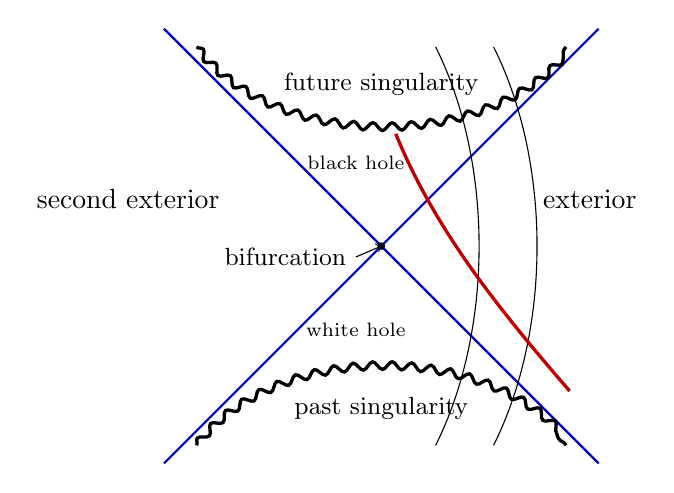
\begin{tikzpicture}[scale=0.92]
\draw[blue!75!black,thick] (-3,-3) -- (3,3);
\draw[blue!75!black,thick] (-3,3) -- (3,-3);
\draw[very thick,decorate,decoration={snake,amplitude=1.4pt,segment length=7pt}]
  (-2.55,2.75) .. controls (-1.45,1.35) and (1.45,1.35) .. (2.55,2.75);
\draw[very thick,decorate,decoration={snake,amplitude=1.4pt,segment length=7pt}]
  (-2.55,-2.75) .. controls (-1.45,-1.35) and (1.45,-1.35) .. (2.55,-2.75);
\draw (0.75,-2.75) .. controls (1.55,-1.15) and (1.55,1.15) .. (0.75,2.75);
\draw (1.55,-2.75) .. controls (2.35,-1.15) and (2.35,1.15) .. (1.55,2.75);
\draw[red!75!black,very thick] (2.6,-2.0) .. controls (1.65,-0.9) and (0.75,0.2) .. (0.2,1.55);
\fill (0,0) circle (1.5pt);
\node[above,font=\small] at (0,1.95) {future singularity};
\node[below,font=\small] at (0,-1.95) {past singularity};
\node[right] at (2.10,0.65) {exterior};
\node[left] at (-2.10,0.65) {second exterior};
\node[font=\scriptsize] at (-0.35,1.15) {black hole};
\node[font=\scriptsize] at (-0.35,-1.15) {white hole};
\node[font=\small,anchor=east] (bifurcation-label) at (-0.35,-0.15) {bifurcation};
\draw[->,thin] (bifurcation-label.east) -- (0,0);
\end{tikzpicture}
\caption{압축하기 전의 인과 그림을 정돈해 나타냈다. 영 지평선은 분기면에서 교차하며, 공간꼴 특이점은 미래 쐐기와 과거 쐐기에 놓인다.}
\end{figure}

\subsection{가능한 일과 전형적인 일}

미시적 역학은 매우 높은 정확도로 시간 반전 대칭이지만, 거시적 이력에는 선호되는 방향이 있다. 폭탄은 쉽게 폭발하지만, 흩어진 파편이 다시 모여 폭탄을 재구성하는 일은 거의 없다. 공은 불안정한 꼭대기에서 쉽게 굴러 떨어지지만, 무작위로 던진 공이 정확히 그곳에 멈추는 일은 거의 없다. 당구공을 삼각형으로 모아 두면 쉽게 흩어지지만, 흩어진 공들이 저절로 삼각형으로 모이는 일은 없다. 뜨거운 물에서는 얼음이 녹지만, 물이 새 얼음 덩어리를 만들어 내보내는 일은 거의 없다.

이 차이를 만드는 것은 엔트로피다. 낮은 엔트로피의 거시상태는 위상공간에서 아주 작은 영역만 차지하지만, 높은 엔트로피의 거시상태에는 어마어마하게 많은 미시적 배열이 들어 있다. 방정식은 시간 반전된 궤적도 허용하지만, 그 궤적의 초기 미시상태를 준비하려면 믿기 어려울 만큼 정밀한 상관관계를 갖춰야 한다.

\begin{classroomqa}
\audiencequestion{흩어진 각각의 정확한 배열도 그에 대응하는 정확한 시간 반전 배열만큼이나 가능성이 낮지 않나요?\lecturetimestamp{00:56:55}}
\lecturerresponse{개별적으로 지정된 미시상태끼리 비교한다면 그렇다. 비대칭성은 거시상태끼리 비교할 때 나타난다. 흩어진 배열에 해당하는 미시상태는 정확히 모아 놓은 당구공 삼각형에 해당하는 미시상태보다 훨씬 많으므로, 전자의 설명에 부합하는 미시상태 대부분은 거시적으로 무질서한 상태에 머문다.}
\end{classroomqa}

완전히 질서 있게 배열된 앨리스를 방출하는 화이트홀은 엔트로피가 감소하는 이력의 중력적 사례다. 가역 방정식이 허용하기는 하지만, 극도로 특별한 과거를 필요로 한다. 지평선에는 엔트로피와 감춰진 미시 정보가 있으므로 앨리스 크기의 요동이 논리적으로 금지되는 것은 아니다. 다만 그 가능성은 압도적으로 억제된다.

\begin{classroomqa}
\audiencequestion{그런 요동은 양자적일까요, 열적일까요?\lecturetimestamp{00:59:48}}
\lecturerresponse{두 종류 모두 기여할 수 있다. 보통의 뜨거운 계에서는 열적 요동이라는 표현이 주된 설명이지만, 블랙홀에서는 양자 효과와 열 효과가 서로 얽혀 있다. 어느 경우든 핵심은 엔트로피에 따른 억제다.}
\end{classroomqa}

\section{고유거리와 펜로즈 압축}

전역 시공간을 그리기 전에 반지름과 관련된 용어를 정확히 하자. 고유시간은 시간꼴 세계선을 따라 시계가 측정하는 시간이다. 고유거리는 선택한 공간꼴 곡선을 따라 국소적인 자를 이어 재는 거리다. 슈바르츠실트 시간 일정 절편 \(t\)에서는
\begin{equation}
d\rho=\frac{dr}{\sqrt{1-2GM/r}}.
\label{eq:l04-proper-distance}
\end{equation}
이다. 따라서 \(r\)는 면적반지름 좌표이지, 지평선에서 잰 직접적인 자의 거리와는 다르다.

이제 반지름 방향의 평탄한 시공간에서 시작하자. \(t\)와 \(\rho\ge0\)만 남긴다. 선 \(\rho=0\)은 공간적 원점이다. 원점으로 들어오는 반지름 방향 광선은 반대편의 물리적 공간으로 계속 나아가며, 축약된 반평면에서는 반사되어 나오는 것처럼 보인다.

펜로즈 도표는 \(t\)와 \(\rho\)의 모든 유한값과 무한값을 유한한 영역에 대응시키면서 영 방향을 보존한다. 두 가지 규칙은 다음과 같다.
\begin{enumerate}
\item 시공간 전체를 유한한 영역으로 압축한다.
\item 반지름 방향 광선을 \(45^\circ\)로 유지한다.
\end{enumerate}
길이와 일반적인 각도는 왜곡되지만 인과 관계는 보존된다.

\begin{figure}[htbp]
\centering
\includegraphics[width=0.70\textwidth]{lecture_04_figure_06.png}
\caption{반지름 방향 민코프스키 시공간을 압축한 격자. 무한한 과거와 미래는 왼쪽 위아래 끝점에 놓이며, 무한한 반지름은 오른쪽 꼭짓점으로 압축된다.}
\lectureframe{01:14:44.040}
\end{figure}

\begin{figure}[htbp]
\centering
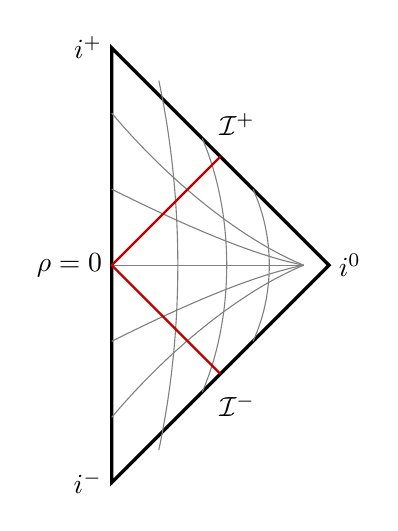
\begin{tikzpicture}[scale=0.92]
\coordinate (im) at (0,-3);
\coordinate (ip) at (0,3);
\coordinate (iz) at (3,0);
\draw[very thick] (im) -- (ip) -- (iz) -- cycle;
\draw[gray] (0,-2.1) .. controls (0.8,-1.15) and (1.8,-0.35) .. (2.65,0);
\draw[gray] (0,-1.05) .. controls (0.9,-0.6) and (1.9,-0.15) .. (2.65,0);
\draw[gray] (0,0) -- (2.65,0);
\draw[gray] (0,1.05) .. controls (0.9,0.6) and (1.9,0.15) .. (2.65,0);
\draw[gray] (0,2.1) .. controls (0.8,1.15) and (1.8,0.35) .. (2.65,0);
\draw[gray] (0.65,-2.55) .. controls (1.0,-0.9) and (1.0,0.9) .. (0.65,2.55);
\draw[gray] (1.25,-1.75) .. controls (1.7,-0.7) and (1.7,0.7) .. (1.25,1.75);
\draw[gray] (1.95,-1.05) .. controls (2.25,-0.4) and (2.25,0.4) .. (1.95,1.05);
\draw[red!75!black,thick] (1.5,-1.5) -- (0,0) -- (1.5,1.5);
\node[left] at (ip) {\(i^+\)};
\node[left] at (im) {\(i^-\)};
\node[right] at (iz) {\(i^0\)};
\node[above right] at (1.35,1.65) {\(\mathcal{I}^+\)};
\node[below right] at (1.35,-1.65) {\(\mathcal{I}^-\)};
\node[left] at (0,0) {\(\rho=0\)};
\end{tikzpicture}
\caption{유한한 삼각형 안에 나타낸 반지름 방향 민코프스키 시공간. 빨간 영선은 \(\mathcal{I}^-\)에서 들어와 원점에 도달한 뒤 \(\mathcal{I}^+\)를 통해 나간다.}
\label{fig:l04-flat-penrose}
\end{figure}

각 끝점은 서로 다른 인과적 의미를 갖는다.
\begin{equation}
\begin{aligned}
i^-&:\ \text{past timelike infinity},\\
i^+&:\ \text{future timelike infinity},\\
i^0&:\ \text{spatial infinity},\\
\mathcal{I}^-&:\ \text{past null infinity},\\
\mathcal{I}^+&:\ \text{future null infinity}.
\end{aligned}
\end{equation}
기호 \(\mathcal{I}^{-}\)와 \(\mathcal{I}^{+}\)는 각각 스크라이 마이너스와 스크라이 플러스로 읽는다.

\begin{classroomqa}
\audiencequestion{왜곡된 격자 칸의 모서리들을 통과하려면 영선이 모든 칸의 꼭짓점을 지나며 조금 휘어야 하나요?\lecturetimestamp{01:11:08}}
\lecturerresponse{좌표 격자 전체를 정확히 그리면 그 교점들은 영곡선과 일관되게 놓인다. 핵심 구성은 등각적이다. 고정 \(t\)선과 고정 \(\rho\)선이 휘고 빽빽해져도 반지름 방향의 영방향은 \(45^\circ\)를 유지한다.}
\end{classroomqa}

\begin{classroomqa}
\audiencequestion{원점을 비껴 가는 광선은 어떻게 그려지나요?\lecturetimestamp{01:11:45}}
\lecturerresponse{최단 접근 거리는 0이 아니며, 광선은 다시 바깥쪽으로 나아갑니다. 각운동을 고려하면 방사 방향으로 투영한 경로가 단일한 \(45^\circ\) 직선일 필요는 없습니다.}
\end{classroomqa}

\begin{classroomqa}
\audiencequestion{그렇다면 그 광선은 왜 \(45^\circ\)가 아닌가요?\lecturetimestamp{01:12:49}}
\lecturerresponse{\(45^\circ\) 규칙은 반지름 방향 광선에 대해 말한 것이다. 각운동량을 가진 영선은 운동의 일부를 각방향에 사용하므로, \(t\)-\(\rho\) 평면에 투영한 경로는 반지름 방향이 아니다.}
\end{classroomqa}

\section{영원한 슈바르츠실트 도표}

압축된 도표에는 네 영역이 있다. 양쪽의 마름모 영역은 점근적으로 평탄한 외부 영역이다. 위쪽 삼각형은 블랙홀 내부이며 미래의 공간꼴 특이점에서 끝난다. 아래쪽 삼각형은 화이트홀 영역이며 과거의 공간꼴 특이점에서 시작한다. 이 영역들을 합치면 최대 연장된 슈바르츠실트 기하학이 된다.

\begin{figure}[htbp]
\centering
\includegraphics[width=0.74\textwidth]{lecture_04_figure_07.png}
\caption{특이점, 지평선, 영 궤적, 그리고 한쪽 점근 경계를 표시한 영원한 슈바르츠실트 펜로즈 도표.}
\lectureframe{01:21:30.000}
\end{figure}

\begin{figure}[htbp]
\centering
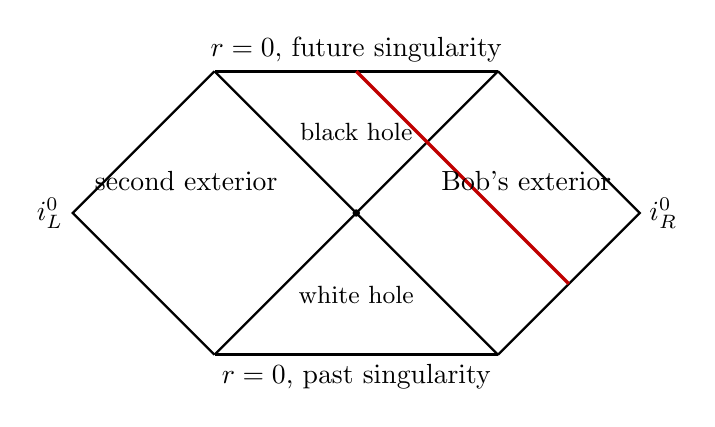
\begin{tikzpicture}[scale=0.90]
\coordinate (C) at (0,0);
\coordinate (TL) at (-2,2);
\coordinate (TR) at (2,2);
\coordinate (BL) at (-2,-2);
\coordinate (BR) at (2,-2);
\coordinate (L) at (-4.0,0);
\coordinate (R) at (4.0,0);
\draw[very thick] (TL) -- (TR);
\draw[very thick] (BL) -- (BR);
\draw[thick] (C) -- (TL) (C) -- (TR) (C) -- (BL) (C) -- (BR);
\draw[thick] (TL) -- (L) -- (BL);
\draw[thick] (TR) -- (R) -- (BR);
\draw[red!75!black,very thick] (3,-1) -- (1,1) -- (0,2);
\node[above] at (0,2) {\(r=0\), future singularity};
\node[below] at (0,-2) {\(r=0\), past singularity};
\node[font=\small] at (0,1.15) {black hole};
\node[font=\small] at (0,-1.15) {white hole};
\node at (2.4,0.45) {Bob's exterior};
\node at (-2.4,0.45) {second exterior};
\node[right] at (R) {\(i^0_R\)};
\node[left] at (L) {\(i^0_L\)};
\fill (C) circle (1.5pt);
\end{tikzpicture}
\caption{영원한 슈바르츠실트 시공간의 네 영역. 안쪽으로 향하는 반지름 방향 광선은 미래 지평선을 통과해 \(r=0\)에서 끝난다.}
\label{fig:l04-eternal}
\end{figure}

\(\mathcal{I}^-\)에서 시작한 안쪽 방향 반지름 광선은 미래 지평선을 통과해 특이점에서 끝난다. 위쪽 삼각형의 인과곡선은 모두 같은 종말을 맞는다. 두 번째 외부 영역은 흔히 아인슈타인--로젠 다리의 반대쪽 입구라고 설명하지만, 통과할 수는 없다. 한 외부 영역에서 다른 영역으로 인과적으로 이동하려 하면 블랙홀 영역에 들어가 특이점에 이른다.

\begin{classroomqa}
\audiencequestion{두 외부 세계는 웜홀로 연결되어 있나요? 그 웜홀을 통해 신호를 보낼 수 있나요?\lecturetimestamp{01:22:21}}
\lecturerresponse{적절한 공간 절편에서 보면 영원한 기하학에는 아인슈타인--로젠 다리가 있지만, 어느 인과 신호도 한 외부 영역에서 다른 영역으로 건너가지 못한다. 다리가 너무 빨리 오므라들기 때문이다. 지평선에 들어간 빛조차 미래 특이점에서 끝난다.}
\end{classroomqa}

이 도표는 태초부터 존재해 온 블랙홀을 나타낸다. 실제 천체물리학적 블랙홀은 물질의 붕괴로 형성된다. 그 인과도에는 과거 화이트홀 특이점도 두 번째 점근 외부 영역도 없다. 이 기하학을 구성하려면 구형 껍질을 이해해야 한다.

\section{붕괴로 블랙홀 만들기}

안쪽으로 들어오는 입자들이 이루는 확산된 구형 껍질을 생각해 보자. 입자는 광자일 수도 있다. 에너지도 중력을 작용시키므로, 충분히 집중된 복사 펄스는 블랙홀을 만들 수 있다. 붕괴 전에는 중심 영역이 빈 평탄 시공간과 비슷하고, 에너지가 충분히 압축된 뒤에는 외부가 슈바르츠실트 시공간과 비슷해진다. 문제는 움직이는 껍질을 경계로 두 영역을 이어 붙이는 것이다.

\subsection{뉴턴의 껍질 정리}

총질량이 \(M\)인 구대칭 뉴턴 껍질의 경우, 중력에 대한 가우스 법칙은 다음과 같습니다.
\begin{equation}
\oint \mathbf{g}\cdot d\mathbf{A}=-4\pi G M_{\mathrm{enc}}.
\label{eq:l04-gauss-gravity}
\end{equation}
구대칭이므로 \(\mathbf{g}=g(r)\hat{\mathbf r}\),
\begin{equation}
g(r)=
\begin{cases}
0, & r<R_{\mathrm{shell}},\\[4pt]
-\dfrac{GM}{r^2}, & r>R_{\mathrm{shell}}.
\end{cases}
\label{eq:l04-shell-field}
\end{equation}
껍질 내부에는 포함된 질량이 없으므로 중력장은 사라집니다. 껍질 외부에서는 중심에 점질량 \(M\)이 있는 경우와 중력장이 정확히 같습니다. 내부 퍼텐셜은 0이 아니라 일정하지만, 국소적인 뉴턴 힘은 남지 않습니다.\editorialnote{강의실에서 제시한 장선 논증은 가우스 법칙으로 정확히 표현됩니다. 장이 0인 것과 퍼텐셜이 일정한 것은 상대론에서 시계의 정규화를 비교할 때 중요합니다.}

총질량이 보존되는 한 완벽한 구형 껍질이 수축하는 동안에도 이 결론은 성립한다. 변하는 것은 내부 해와 외부 해 사이 경계의 위치뿐이다.

\subsection{버코프 정리}

이에 대응하는 상대론적 결과는 버코프 정리다. 모든 구대칭 진공 영역은 국소적으로 슈바르츠실트 해족의 한 부분이다. 중심에 질량이 없는 껍질의 경우,
\begin{align}
ds^2_{\mathrm{inside}}&=-dT^2+dR^2+R^2d\Omega_2^2,\\
ds^2_{\mathrm{outside}}&=
-\left(1-\frac{2GM}{r}\right)dt^2
\nonumber\\
&\quad+\frac{dr^2}{1-2GM/r}
+r^2d\Omega_2^2.
\label{eq:l04-birkhoff-pieces}
\end{align}

\begin{figure}[htbp]
\centering
\includegraphics[width=0.74\textwidth]{lecture_04_figure_08.png}
\caption{껍질 경계에서 해를 이어 붙이는 칠판 그림: 원 안쪽은 평탄한 시공간이고 바깥쪽은 슈바르츠실트 해다.}
\lectureframe{01:34:15.000}
\end{figure}

\begin{classroomqa}
\audiencequestion{일반상대론에서 구형 껍질 바깥에는 어떤 계량이 나타나나요?\lecturetimestamp{01:33:17}}
\lecturerresponse{껍질의 보존된 총질량과 같은 질량 매개변수를 갖는 슈바르츠실트 계량이다. 비어 있는 중심 영역은 국소적으로 민코프스키 시공간이다.}
\end{classroomqa}

\begin{classroomqa}
\audiencequestion{껍질이 수축해도 질량 매개변수가 변하지 않는 이유는 무엇인가요?\lecturetimestamp{01:34:33}}
\lecturerresponse{총에너지가 보존되기 때문이다. 껍질의 반지름과 운동에너지 또는 결합에너지에 따른 기여는 변할 수 있지만, 고립된 구대칭 계의 보존되는 외부 질량은 고정되어 있다. 움직이는 껍질은 평탄 영역과 슈바르츠실트 영역이 만나는 위치를 바꾼다.}
\end{classroomqa}

내부가 평탄하다고 해서 내부 시계의 시간 정규화가 무한대에서의 시계와 반드시 같다는 뜻은 아니다. 껍질을 가로질러 접합하면 내부 시간 좌표에 상수가 곱해질 수 있으며, 껍질이 움직이는 경우에는 그에 맞는 접합 조건이 필요하다.\editorialnote{비르코프 정리는 각 진공 영역을 국소적으로 결정한다. 두 영역 좌표 사이의 전역적 관계는 껍질을 가로질러 유도 계량과 외재 곡률을 접합함으로써 정해진다. 이러한 세부 사항은 다음 강의에서 다룰 붕괴 구성과 마찬가지로 여기서는 미룬다.}

이제 블랙홀 형성에 필요한 두 부분, 즉 수축하는 껍질 안쪽의 민코프스키 시공간과 바깥쪽의 슈바르츠실트 시공간을 갖추었다. 껍질이 안쪽으로 움직이면 두 영역의 경계가 세계관을 이룬다. 이 경계를 슈바르츠실트 반지름을 통과해 따라가면 그림~\ref{fig:l04-eternal}의 비물리적인 과거 부분은 규칙적인 붕괴 전 영역으로 대체되고, 실제 블랙홀의 사건의 지평선이 어디서 시작되는지도 드러난다.
